\subsubsection{Menú 01: Principal} \label{mn01}
 \begin{center}
   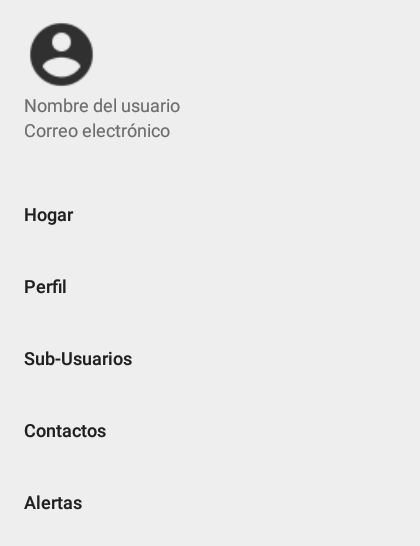
\includegraphics[scale=.25]{Capitulo3/img/menu/MN_01_(1).png} \\
   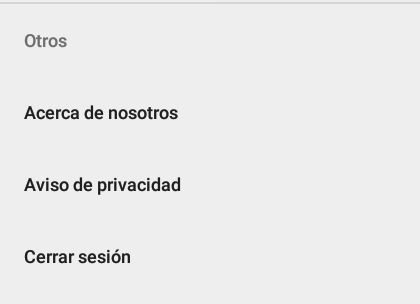
\includegraphics[scale=.25]{Capitulo3/img/menu/MN_01_(2).png}
   \captionof{figure}{\nameref{mn01}}
   \label{fig:mn01_fig}
 \end{center}

 \begin{itemize}
   \item \textit{Hogar}: Opción que lleva a la vista \textbf{\ref{iu07}}.
   \item \textit{Perfil}: Opción que lleva a la vista \textbf{\ref{iu0}} donde puede consultar su perfil.
   \item \textit{Sub-Usuarios}:  Opción que lleva a la vista \textbf{\ref{iu0}} se pueden ver los sub-usuarios que tiene registrados bajo su cuenta.
   \item \textit{Contactos}:  Opción que lleva a la vista \textbf{\ref{iu0}} donde puede consultar todos los contactos de emergencia que tiene registrados.
   \item \textit{Alertas}:  Opción que lleva a la vista \textbf{\ref{iu0}} donde puede visualizar las alertas actuales o pasadas.
   \item \textit{Otros}
     \begin{itemize}
       \item \textit{Acerca de nosotros}:  Opción que muestra la vista con la información de los desarroladores.
       \item \textit{Aviso de privacidad}:  Opción que muestra el aviso de privacidad del sistema.
       \item \textit{Cerrar sesión}:  Opción que términa la sesión del usuario.
     \end{itemize}
 \end{itemize}